
\documentclass{article}
\usepackage{amsmath}
\usepackage{tikz}
\title{Statistics 371 Homework 1}
\author{Jordan Paldino}
\date{18 January 2018}
\begin{document}
\begin{enumerate}
\item \textit{Page 12 Problem 1:} \\
\begin{enumerate}
\item New York Times, Wall Street Journal, The Daily Reflector, Los Angelas Times \\
\item Apple, Microsoft, IBM, AMD \\
\item Jordan Paldino, Nathan Chen, Mathew Blizzard, Martin Shank \\
\item 4.0, 2.7, 3.0, 1.9 \\
\end{enumerate}
\item Question 2\\
\begin{enumerate}
\item \begin{tabular}{l|l }
\textbf{00}0. & 00\textbf{0} \\ \hline
$32$ & 5 5\\
$33$ & \\
34 & 4 \\
35 & 6 6 9 9 \\
36 & 3 4 4 6 9 \\
37 & 0 3 3 4 5 \\
38 & 9 \\
39 & 2 3 4 7 \\
40 & 2 3 \\
41 &  \\
42 & 4\\
\end{tabular} \\
\item Mean=$$\frac{\sum\limits_{i=1}^{n} x_i}{n}= \frac{9638}{26}=370.69$$ \\
Median=$371.5$ \\
\item The Median could not be affected by increasing the value. This is because the median value is determined by the location relative to the other values, and since 424 is the largest value, the median cannot be increased.\\
Decreasing the value, however, the largest value could be decreased by 51. This is because this brings the largest point down to the value which is factored into the median.
\item  $\widetilde{x}=370.69 seconds. In order t translate the value into seconds, we take the value we solved for and divide by 60, which results in 6.18 minutes. As for median, we can do the same thing with 371.5 seconds, changing it to 6.19 minutes.$
\end{enumerate}
\item Page 44 Problem 45:
\begin{enumerate}
\item  $Varience=\frac{\sum\limits_{i=1}^n (x_i-\bar{x})^2}{n}=1933.11$\\
Deviation=$\sqrt{Varience}=43.97$
\item In order to find the value in hours, we must first consider the units which the above values are in. The standard varience is in $min^2$, meaning that in order to convert this value into hours, we must divide by $60^2, or 3600, making the standard variation .54 hours$. We can simply divide the deviation by 60 since the units are minutes, giving us .73 hours. 
\end{enumerate}
\item Page 57 Problem 3
\begin{enumerate}
\item The outcomes 1 sucess and 2 sucess 3 failure, 1 sucess 2 failure 3 success are in A.
\item The outcomes 1 sucess 2 sucess 3 failure, and 1 sucess 2 failure 3 success, and 1 success 2 sucess 3 sucess are in B.
\item All values in B are in C
\item C': 1 failure, 2 failure, 3 failure, and 1 failure, 2 failure, 3 success, and 1 failure 2 success 3 success, and 1 failure, 2 success, 3 failure, and 1 sucess 2 failure 3 failure. \\
  A $\cup$ C: The outcomes 1 sucess and 2 sucess 3 failure, 1 sucess 2 failure 3 success. \\
  A $\cap$ C: The outcomes 1 sucess and 2 sucess 3 failure, 1 sucess 2 failure 3 success. \\
  B $\cup$ C: The outcomes 1 sucess 2 sucess 3 failure, and1 sucess 2 failure 3 success, and 1 success 2 sucess 3 success. \\
  B $\cap$ C: The outcomes 1 sucess and 2 sucess 3 failure, 1 sucess 2 failure 3 success.

\end{enumerate}
\item
\begin{center} 
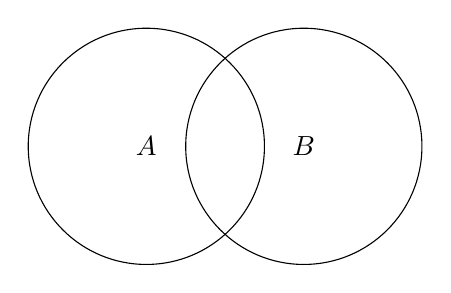
\begin{tikzpicture}
\draw (-1,0) circle (1.5cm) node {$A$};
\draw (1,0) circle (1.5cm) node {$B$};
\end{tikzpicture}
\end{center}
\end{enumerate}
\end{document}
